%%%%%%%%%%%%%%%%%%%%%%%%%%%%%%%%%%%%%%%%%

% Template license:
% CC BY-NC-SA 3.0 (http://creativecommons.org/licenses/by-nc-sa/3.0/)
%
%%%%%%%%%%%%%%%%%%%%%%%%%%%%%%%%%%%%%%%%%

%----------------------------------------------------------------------------------------
%	PACKAGES AND OTHER DOCUMENT CONFIGURATIONS
%----------------------------------------------------------------------------------------

\documentclass[
12pt, % The default document font size, options: 10pt, 11pt, 12pt
%oneside, % Two side (alternating margins) for binding by default, uncomment to switch to one side
english, % ngerman for German
%singlespacing, % Single line spacing, alternatives: onehalfspacing or doublespacing
%draft, % Uncomment to enable draft mode (no pictures, no links, overfull hboxes indicated)
%nolistspacing, % If the document is onehalfspacing or doublespacing, uncomment this to set spacing in lists to single
%liststotoc, % Uncomment to add the list of figures/tables/etc to the table of contents
%toctotoc, % Uncomment to add the main table of contents to the table of contents
%parskip, % Uncomment to add space between paragraphs
%nohyperref, % Uncomment to not load the hyperref package
%headsepline, % Uncomment to get a line under the header
%chapterinoneline, % Uncomment to place the chapter title next to the number on one line
%consistentlayout, % Uncomment to change the layout of the declaration, abstract and acknowledgements pages to match the default layout
]{report} % The class file specifying the document structure

\usepackage[utf8]{inputenc} % Required for inputting international characters
\usepackage[T1]{fontenc} % Output font encoding for international characters

\usepackage{graphicx}
\usepackage{hyperref}

\usepackage{tikz}
\usetikzlibrary{shapes.geometric, arrows}

\usepackage{booktabs} % for tables
\usepackage{mathpazo} % Use the Palatino font by default

\usepackage{tesi} % thesis structure

\usepackage[autostyle=true]{csquotes} % Required to generate language-dependent quotes in the bibliography
\usepackage[english]{babel}

\usepackage{amsmath}

\usepackage{fancyhdr} 
\fancyhf{}
\cfoot{\thepage}
\pagestyle{fancy}

\usepackage{hyperref}

\begin{document}
	
	\title{DeepMiRNA: a novel approach to microRNA \\ 
		target prediction using Deep Learning}
	\author{Simone Sinigaglia}
	\dept{Dipartimento di Informatica}
	\anno{2018/2019}
	\matricola{902960}
	\relatore{Prof. Sebastiano Vigna}
	\correlatore{Prof. Paolo Boldi}
	
	\begin{center}
		
\includegraphics{Figures/logo_unimi}\\[1cm]
	\end{center}
	
	\beforepreface
	I would like to thank \dots
	\afterpreface
	
	\include{Frontpages/Intro}
	
%---------------------------------------------------------------------------------------
%
%	THESIS CONTENT - CHAPTERS
%
%---------------------------------------------------------------------------------------

	% Chapter 1

\chapter{MicroRNAs and their importance in living beings} % Main chapter title

\label{Chapter1} % For referencing the chapter elsewhere, use \ref{Chapter1} 

%----------------------------------------------------------------------------------------

% Define some commands to keep the formatting separated from the content 
\newcommand{\keyword}[1]{\textbf{#1}}
\newcommand{\tabhead}[1]{\textbf{#1}}
\newcommand{\code}[1]{\texttt{#1}}
\newcommand{\file}[1]{\texttt{\bfseries#1}}
\newcommand{\option}[1]{\texttt{\itshape#1}}

%----------------------------------------------------------------------------------------

\section{What are microRNAs?}
MicroRNAs (abbreviated miRNAs) are a family of $\approx 22$-nucleotide small non-coding RNAs that regulates gene expression at the post-transcriptional level \cite{mirna_intro}. This means that they act by binding to partially complementary sites on target genes, which had been previously transcribed from the DNA of the cell, to induce cleavage or repression of productive translation, preventing this way the target gene to be able to exit the cell and start the translational process that produces peptides and proteins.

\begin{figure}[hbt!]
	\centering
	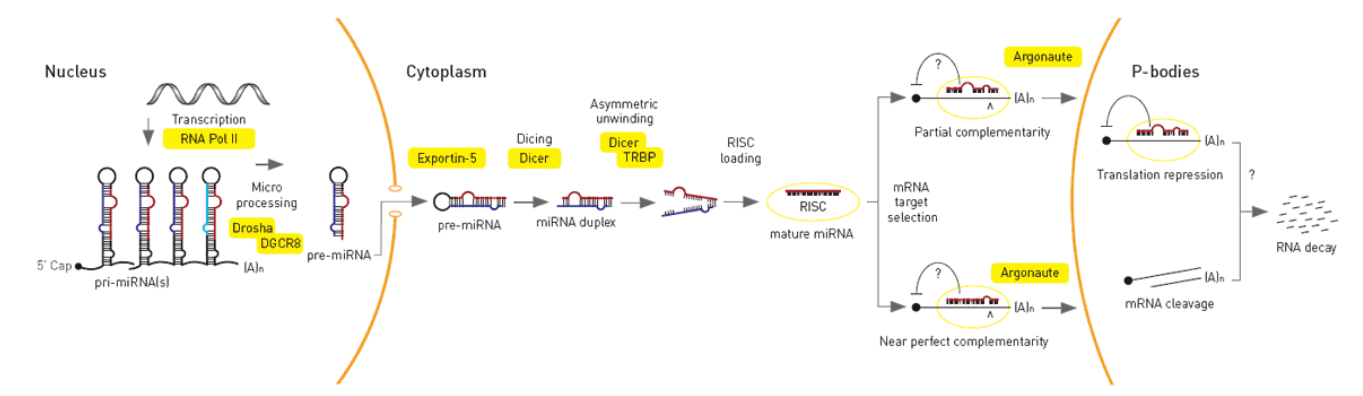
\includegraphics[width=1.0\textwidth]{Figures/mirna_genesis}
	\caption{MiRNAs genesis and functionalities}
	\label{fig:mirna_genesis}
\end{figure}

\subsection{Transcription and processing of miRNAs}
As shown in figure \ref{fig:mirna_genesis} miRNAs genes are transcribed by the RNA polymerase II as as large primary transcripts (pri-miRNA) that are processed by a protein complex containing the enzyme Drosha, to form an approximately 70 nucleotide precursor miRNA (pre-miRNA). This precursor is subsequently transported to the cytoplasm where it is processed by a second enzyme, called DICER, to form a mature miRNA of approximately 22 nucleotides. The mature miRNA is then incorporated into a ribonuclear particle to form the RNA-induced silencing complex, RISC, which mediates gene silencing.

It's important to note that, generally, only one of the two strands of the stem loop is incorporated into the silencing process, and it's selected on the basis of its thermodynamic instability and weaker base-pairing on the 5' end relative to the other strand. The latter, called the passenger strand due to its lower levels in the steady state, is usually denoted with an asterisk (*) and is normally degraded. However, in some cases, both strands of the duplex are viable and become functional miRNAs that target different mRNA populations. (see figure \ref{fig:mirna_stems})

\begin{figure}[hbt!]
	\centering
	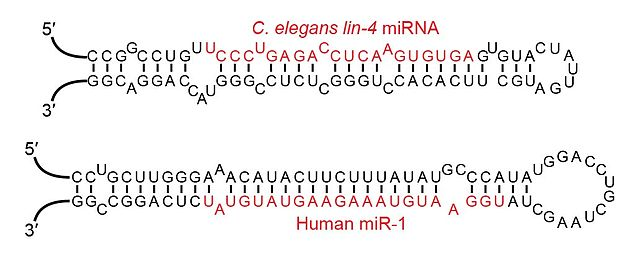
\includegraphics[width=1.0\textwidth]{Figures/mirna_stems}
	\caption{Examples of miRNA stem-loops. In red is shown the mature miRNA}
	\label{fig:mirna_stems}
\end{figure}

\subsection{RNA-induced silencing complex (RISC)}
As mentioned before the mature miRNA is part of an active RNA-induced silencing complex (RISC). This process represents their main functionality in both animals and plants. 
The RISC it is a key process in gene silencing and can act in two different ways as depicted in the right-hand side of picture \ref{fig:mirna_genesis}: via mRNA degradation or by preventing mRNA translation. It has been demonstrated that given complete complementarity between the miRNA and target mRNA sequence, Ago2 can cleave the mRNA and lead to direct mRNA degradation. In the presence of only partial complementarity instead, silencing is achieved by preventing translation \cite{cleavage}.
 
%----------------------------------------------------------------------------------------

\section{Why are they important?}
MiRNAs are particularly abundant in many mammalian cell types and appear to target about 60\% of the genes of humans and other mammals \cite{conserved_pairing}.

Many miRNAs are evolutionarily conserved, which implies that they have important biological functions \cite{conserved_pairing}. For example, 90 families of miRNAs have been conserved since at least the common ancestor of mammals and fish, and most of these conserved miRNAs have important functions.

The discovery of the first miRNA over 20 years ago has ushered in a new era in molecular biology. There are now over 2000 miRNAs that have been discovered in humans and it is believed that they collectively regulate two third of the genes in the genome.

The repressive action of miRNAs has a huge impact on many biological processes such as cell cycle control and several developmental and physiological processes including stem cell differentiation, cardiac and skeletal muscle development, neurogenesis, insulin secretion, cholesterol metabolism, aging, immune responses and viral replication. \cite{mirna_annotation}

In addition to their important roles in healthy individuals, microRNAs have also been implicated in a number of diseases including a broad range of cancers, heart and neurological diseases.  In fact it has been discovered that their expression patterns  are highly specific in respect to external stimuli, developmental stage or tissue and this can be used to diagnose diseases in which the expression levels of miRNAs are known to change considerably \cite{computational_methods}. Consequently, miRNAs are intensely studied as candidates for clinical diagnosis and predictors of drug response \cite{mirna_diseases}.

\section{Why miRNAs target prediction is a difficult task?}




\section{acaso}

\subsection{Folders}

This template comes as a single zip file that expands out to several files and folders. The folder names are mostly self-explanatory:

\keyword{Appendices} -- this is the folder where you put the appendices. Each appendix should go into its own separate \file{.tex} file. An example and template are included in the directory.

\keyword{Chapters} -- this is the folder where you put the thesis chapters. A thesis usually has about six chapters, though there is no hard rule on this. Each chapter should go in its own separate \file{.tex} file and they can be split as:
\begin{itemize}
\item Chapter 1: Introduction to the thesis topic
\item Chapter 2: Background information and theory
\item Chapter 3: (Laboratory) experimental setup
\item Chapter 4: Details of experiment 1
\item Chapter 5: Details of experiment 2
\item Chapter 6: Discussion of the experimental results
\item Chapter 7: Conclusion and future directions
\end{itemize}

%---------------------------------------------------------------------------------------

\subsection{Tables}

Tables are an important way of displaying your results, below is an example table which was generated with this code:

{\small
\begin{verbatim}
\begin{table}
\caption{The effects of treatments X and Y on the four groups studied.}
\label{tab:treatments}
\centering
\begin{tabular}{l l l}
\toprule
\tabhead{Groups} & \tabhead{Treatment X} & \tabhead{Treatment Y} \\
\midrule
1 & 0.2 & 0.8\\
2 & 0.17 & 0.7\\
3 & 0.24 & 0.75\\
4 & 0.68 & 0.3\\
\bottomrule\\
\end{tabular}
\end{table}
\end{verbatim}
}

\begin{table}
\caption{The effects of treatments X and Y on the four groups studied.}
\label{tab:treatments}
\centering
\begin{tabular}{l l l}
\toprule
\tabhead{Groups} & \tabhead{Treatment X} & \tabhead{Treatment Y} \\
\midrule
1 & 0.2 & 0.8\\
2 & 0.17 & 0.7\\
3 & 0.24 & 0.75\\
4 & 0.68 & 0.3\\
\bottomrule\\
\end{tabular}
\end{table}

You can reference tables with \verb|\ref{<label>}| where the label is defined within the table environment. See \file{Chapter1.tex} for an example of the label and citation (e.g. Table~\ref{tab:treatments}).


There are many different \LaTeX{} symbols to remember, luckily you can find the most common symbols in \href{http://ctan.org/pkg/comprehensive}{The Comprehensive \LaTeX~Symbol List}.

You can write an equation, which is automatically given an equation number by \LaTeX{} like this:
\begin{verbatim}
\begin{equation}
E = mc^{2}
\label{eqn:Einstein}
\end{equation}
\end{verbatim}


All equations you write (which are not in the middle of paragraph text) are automatically given equation numbers by \LaTeX{}. If you don't want a particular equation numbered, use the unnumbered form:
\begin{verbatim}
\[ a^{2}=4 \]
\end{verbatim}

%----------------------------------------------------------------------------------------

\section{In Closing}

You have reached the end of this mini-guide. You can now rename or overwrite this pdf file and begin writing your own \file{Chapter1.tex} and the rest of your thesis. The easy work of setting up the structure and framework has been taken care of for you. It's now your job to fill it out!

Good luck and have lots of fun!

\begin{flushright}
Guide written by ---\\
Sunil Patel: \href{http://www.sunilpatel.co.uk}{www.sunilpatel.co.uk}\\
Vel: \href{http://www.LaTeXTemplates.com}{LaTeXTemplates.com}
\end{flushright}

	% Chapter 2

\chapter{MicroRNAs target prediction computational methods} % Main chapter title

\label{Chapter2} % For referencing the chapter elsewhere, use \ref{Chapter2} 


%----------------------------------------------------------------------------------------

\section{Introduction}
Earlier in Chapter~\ref{Chapter1} we described how miRNAs play a fundamental role in gene regulation. It is common belief that the final and probably most relevant step in their regulatory pathway is targeting \cite{computational_methods}. Targeting is intended as the binding of the mature miRNA to the messenger RNA via the RNA Induced Silencing Complex (see figure \ref{fig:mirna_binding}). Hence, valid targets need to be identified for miRNAs in order to properly understand their role in cellular pathways. 

However, many of the discovered miRNAs do not yet have identified targets. This is especially the case in animals where the miRNA does not bind to its target with a nearly perfect matching as it does in plants \cite{perfect_matching}. Experiments have proved that a single miRNA has the potential to regulate hundreds of target mRNAs and multiple miRNAs may compete for the regulation of the same mRNA \cite{multiple_binds}, however target validation is difficult, expensive, and time consuming. Thus, having considered all these facts, it is of crucial importance to have accurate computational miRNA target predictions.

\begin{figure}[hbt!]
	\centering
	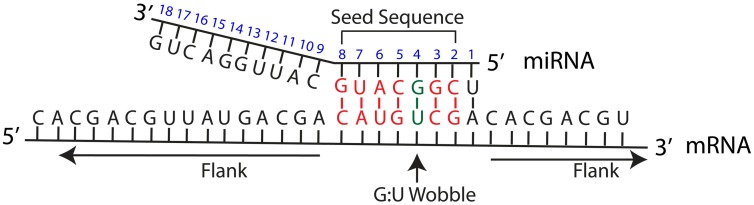
\includegraphics[width=0.7\textwidth]{Figures/seed_match}
	\caption{Example of miRNA targeting.}
	\label{fig:mirna_binding}
\end{figure}

%----------------------------------------------------------------------------------------

\section{MiRNA target prediction}
Before miRNA target prediction tools were available, possible miRNA binding sites were
determined manually. These target sites were later confirmed by laborious and inefficient techniques such as site-directed mutagenesis and other experimental methods. The identification of the first targets for the let-7 and lin-4 miRNAs led to the idea that miRNAs have a pattern in targeting genes which could be used to develop target prediction algorithms \cite{first_predictions}.

Originally gene targeting by miRNAs was believed to be the result of their binding to the 3'UTR of the target mRNA \cite{multiple_binds}, however recent studies \cite{grosswendt} have confirmed gene regulation as a result of the binding of the miRNA to the coding region as well as to the 5'UTR. Furthermore, computational evidence suggests that regulation via the binding of the miRNA to the coding region differs in comparison to the binding pattern seen at the 3'UTR. In particular, it's suggested that miRNAs target the coding regions of mRNAs with short 3'UTRs \cite{functional_sites}.

Another key factor in target prediction is that 3'UTRs are prone to change under different conditions which might result in the elimination of the target site. Binding in the coding region on the other hand may instead present an evolutionary advantage for the cell as it could help in the preservation of the miRNA binding site \cite{mirna_targets}. 

\subsection{Features and methodologies}
While many miRNA targets have been computationally predicted only a limited number
have been experimentally validated. Moreover, although a variety of miRNA target prediction algorithms are implemented, results amongst them are generally inconsistent and correctly identifying functional miRNA targets remains a challenging task.

The various methodologies implemented use several different approaches and analyze a wide range of features for this task, however, the most common characteristics are \cite{common_features}:
\begin{itemize}
	\item seed region complementarity
	\item free energy
	\item site accessibility
	\item conservation
\end{itemize}

\subsubsection{The seed region}
Targeting patterns are very different between plants and animals. Plants, in fact, show a near perfect complement between their miRNA and the respective target mRNA. On the other hand animal miRNAs bind their targets with only partial complementarity. In particular, a region of about 6 to 8 nucleotides in length at the beginning of the miRNA is of crucial importance in the targeting.  This short subsequence is called \emph{seed region} and it comprises the nucleotides between the second at the eighth (the seed sequence in Figure \ref{fig:mirna_binding}) starting from the 5' end. 
The seed region is very important because it binds to the target mRNA leading to the regulation of the gene in question \cite{mirna_overview}.

Undoubtedly the seed region is one of the most commonly used miRNA traits for target prediction. This seed-centric view, in fact,  has been supported by structural studies \cite{structural_basis} and a widely cited report  \cite{canonical_target} that investigated the importance of other (non-canonical) regions within a miRNA concluding that their contributions had relatively low relevance compared to the (canonical)
seed region. More recent experiments, however, have highlighted a role for the entire miRNA, suggesting that a more flexible methodology is needed \cite{helwak}.

\begin{figure}[hbt!]
	\centering
	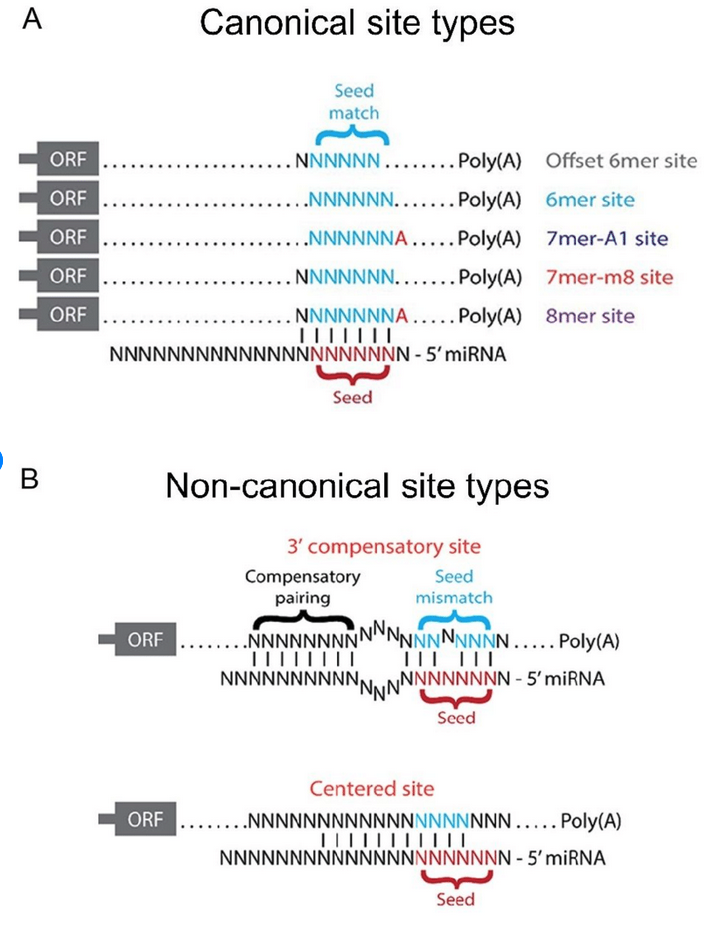
\includegraphics[width=0.5\textwidth]{Figures/canonical_noncanonical}
	\caption{Example of canonical and non-canonical binding sites.}
	\label{fig:canonical_binding}
\end{figure}

\subsubsection{Free energy}
The free energy, also called hybridization energy,  is defined as the energy released by the pairing between the miRNA and mRNA and it can be used as the measure of the stability of the bond. In fact a stable bond is considered more likely to be a functional target of the miRNA. However, since measuring this quantity directly is difficult, usually the change of free energy during a reaction is considered ($\Delta G$). Reactions with a negative $\Delta G$ have less energy available to react in the future, hence they result in systems with an increased stability. By predicting how the miRNA and its candidate target hybridize, regions of high and low free energy can be inferred (Figure \ref{fig:free_energy}) and the overall $\Delta G$ can be used as an indicator of how strongly bound they are \cite{free_energy_survey}.

\begin{figure}[hbt!]
	\centering
	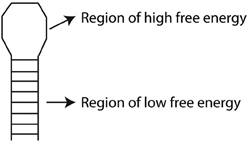
\includegraphics[width=0.5\textwidth]{Figures/free_energy}
	\caption{A hairpin loop is shown with the loop corresponding to a region of high free energy (a positive $\Delta G$) and the stem corresponding to a region of low free energy (a negative $\Delta G$)}
	\label{fig:free_energy}
\end{figure}

\subsubsection{Site accessibility}
Site accessibility is the measure of the ease with which a miRNA can locate and hybridize with its target. After transcription, in fact,  a mRNA assumes a certain secondary structure which can interfere with the miRNA ability to bind to its target site. To understand why this is important, we need to consider that the miRNA:mRNA hybridization involves  a two-step process in which a miRNA firstly binds to a short accessible region of the mRNA and only after, while the secondary structure of the mRNA unfolds, completes the binding.  It is likely that secondary structures contribute to target recognition, because there is an energetic cost to freeing base-pairing interactions within mRNA in order to make the target accessible for miRNA binding. Hence, to assess the likelihood that a mRNA is a target of a given miRNA, the predicted amount of energy required to make the site accessible (the so called site accessibility energy SAE) should be taken into consideration \cite{accessibility_nrg_role}.

The SAE	can be computed as the difference between the free energy cost of opening the mRNA and free energy gained from the intermolecular interaction (Figure \ref{fig:opening_energy}).

\begin{figure}[hbt!]
	\centering
	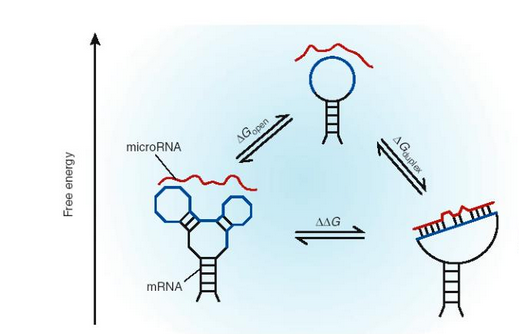
\includegraphics[width=0.7\textwidth]{Figures/opening_energy}
	\caption{Binding of a miRNA to its target mRNA is depicted as a 2-step process. Portion of the mRNA structure must be open before miRNA:mRNA base pairing can be established.}
	\label{fig:opening_energy}
\end{figure}

\subsubsection{Conservation}
Conservation refers to the maintenance of a sequence across species. According to many reports \cite{computational_methods} looking at conserved targets between different species helps reducing the number of false positive results. However, other more recent studies highlighted the fact that this may also increase the number of false negatively identified targets \cite{conserved_pairing}.
	% Chapter 3

\chapter{MicroRNAs target prediction computational methods} % Main chapter title

\label{Chapter3} % For referencing the chapter elsewhere, use \ref{Chapter3} 


%----------------------------------------------------------------------------------------

\section{Introduction}
Earlier in Chapter~\ref{Chapter2} we described how miRNAs play a fundamental role in gene regulation. It is common belief that the final and probably most relevant step in their regulatory pathway is targeting \cite{computational_methods}. Targeting is intended as the binding of the mature miRNA to the messenger RNA via the RNA Induced Silencing Complex (see figure \ref{fig:mirna_binding}). Hence, valid targets need to be identified for miRNAs in order to properly understand their role in cellular pathways. 

However, many of the discovered miRNAs do not yet have identified targets. This is especially the case in animals where the miRNA does not bind to its target with a nearly perfect matching as it does in plants \cite{perfect_matching}. Experiments have proved that a single miRNA has the potential to regulate hundreds of target mRNAs and multiple miRNAs may compete for the regulation of the same mRNA \cite{multiple_binds}, however target validation is difficult, expensive, and time consuming. Thus, having considered all these facts, it is of crucial importance to have accurate computational miRNA target predictions.

\begin{figure}[hbt!]
	\centering
	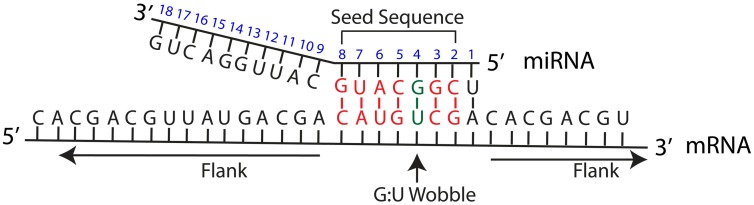
\includegraphics[width=0.7\textwidth]{Figures/seed_match}
	\caption{Example of miRNA targeting.}
	\label{fig:mirna_binding}
\end{figure}

%----------------------------------------------------------------------------------------

\section{MiRNA target prediction}
Before miRNA target prediction tools were available, possible miRNA binding sites were
determined manually. These target sites were later confirmed by laborious and inefficient techniques such as site-directed mutagenesis and other experimental methods. The identification of the first targets for the let-7 and lin-4 miRNAs led to the idea that miRNAs have a pattern in targeting genes which could be used to develop target prediction algorithms \cite{first_predictions}.

Originally gene targeting by miRNAs was believed to be the result of their binding to the 3'UTR of the target mRNA \cite{multiple_binds}, however recent studies \cite{grosswendt} have confirmed gene regulation as a result of the binding of the miRNA to the coding region as well as to the 5'UTR. Furthermore, computational evidence suggests that regulation via the binding of the miRNA to the coding region differs in comparison to the binding pattern seen at the 3'UTR. In particular, it's suggested that miRNAs target the coding regions of mRNAs with short 3'UTRs \cite{functional_sites}.

Another key factor in target prediction is that 3'UTRs are prone to change under different conditions which might result in the elimination of the target site. Binding in the coding region on the other hand may instead present an evolutionary advantage for the cell as it could help in the preservation of the miRNA binding site \cite{mirna_targets}. 

\subsection{Features and methodologies}
While many miRNA targets have been computationally predicted only a limited number
have been experimentally validated. Moreover, although a variety of miRNA target prediction algorithms are implemented, results amongst them are generally inconsistent and correctly identifying functional miRNA targets remains a challenging task.

The average performance of target prediction tools, which typically identify approximately 80\% of known miRNA targets, indicates that the mechanisms associated with miRNA-regulated processes remain poorly understood. Thus, there is a room for novel approaches to improve the knowledge of the rules that govern their targeting process \cite{targeting_rules}

The various methodologies implemented use several different approaches and analyze a wide range of features for this task. Almost all target prediction methods are rule-based or adopt machine learning methodology with varying success. Rule-based systems incorporate various human-crafted descriptors to represent miRNA:gene target binding (e.g. type of pairs in the site, binding stability, or conservation of the target site among species). Machine learning techniques also use those descriptors, but as input features to machine learning models. The limitation of both these approaches is indeed the process of feature selection and representation, which is constrained by
the use of human selected descriptors to model a process that is not fully understood.

The most common characteristics used in miRNA targets identification are \cite{common_features}:
\begin{itemize}
	\item seed region complementarity
	\item free energy
	\item site accessibility
	\item conservation
\end{itemize}

\subsubsection{The seed region}
Targeting patterns are very different between plants and animals. Plants, in fact, show a near perfect complement between their miRNA and the respective target mRNA. On the other hand animal miRNAs bind their targets with only partial complementarity. In particular, a region of about 6 to 8 nucleotides in length at the beginning of the miRNA is of crucial importance in the targeting.  This short subsequence is called \emph{seed region} and it comprises the nucleotides between the second at the eighth (the seed sequence in Figure \ref{fig:mirna_binding}) starting from the 5' end. 
The seed region is very important because it binds to the target mRNA leading to the regulation of the gene in question \cite{mirna_overview}.

Undoubtedly the seed region is one of the most commonly used miRNA traits for target prediction. This seed-centric view, in fact,  has been supported by structural studies \cite{structural_basis} and a widely cited report  \cite{canonical_target} that investigated the importance of other (non-canonical) regions within a miRNA concluding that their contributions had relatively low relevance compared to the (canonical)
seed region. More recent experiments, however, have highlighted a role for the entire miRNA, suggesting that a more flexible methodology is needed \cite{helwak}.

\begin{figure}[hbt!]
	\centering
	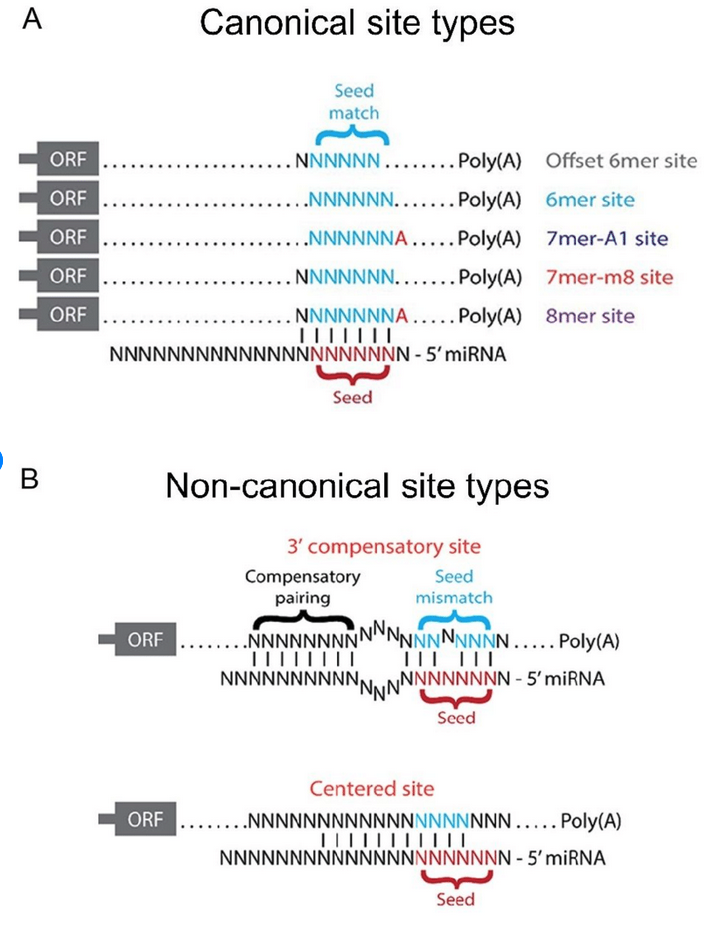
\includegraphics[width=0.5\textwidth]{Figures/canonical_noncanonical}
	\caption{Example of canonical and non-canonical binding sites.}
	\label{fig:canonical_binding}
\end{figure}

\subsubsection{Free energy}
The free energy, also called hybridization energy,  is defined as the energy released by the pairing between the miRNA and mRNA and it can be used as the measure of the stability of the bond. In fact a stable bond is considered more likely to be a functional target of the miRNA. However, since measuring this quantity directly is difficult, usually the change of free energy during a reaction is considered ($\Delta G$). Reactions with a negative $\Delta G$ have less energy available to react in the future, hence they result in systems with an increased stability. By predicting how the miRNA and its candidate target hybridize, regions of high and low free energy can be inferred (Figure \ref{fig:free_energy}) and the overall $\Delta G$ can be used as an indicator of how strongly bound they are \cite{free_energy_survey}. The lower this value the more stable the binding.

\begin{figure}[hbt!]
	\centering
	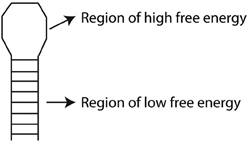
\includegraphics[width=0.5\textwidth]{Figures/free_energy}
	\caption{A hairpin loop is shown with the loop corresponding to a region of high free energy (a positive $\Delta G$) and the stem corresponding to a region of low free energy (a negative $\Delta G$)}
	\label{fig:free_energy}
\end{figure}

\subsubsection{Site accessibility}
Site accessibility is the measure of the ease with which a miRNA can locate and hybridize with its target. After transcription, in fact,  a mRNA assumes a certain secondary structure which can interfere with the miRNA ability to bind to its target site. To understand why this is important, we need to consider that the miRNA:mRNA hybridization involves  a two-step process in which a miRNA firstly binds to a short accessible region of the mRNA and only after, while the secondary structure of the mRNA unfolds, completes the binding.  It is likely that secondary structures contribute to target recognition, because there is an energetic cost to freeing base-pairing interactions within mRNA in order to make the target accessible for miRNA binding. Hence, to assess the likelihood that a mRNA is a target of a given miRNA, the predicted amount of energy required to make the site accessible (the so called site accessibility energy SAE) should be taken into consideration \cite{accessibility_nrg_role}.

The SAE	can be computed as the difference between the free energy cost of opening the mRNA and free energy gained from the intermolecular interaction (Figure \ref{fig:opening_energy}).

\begin{figure}[hbt!]
	\centering
	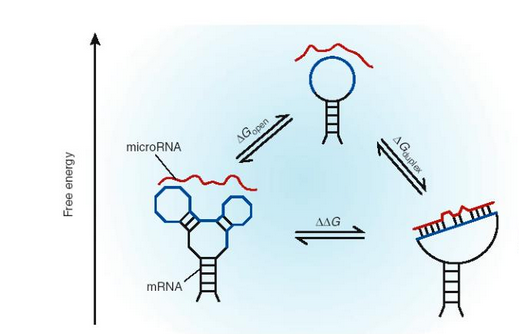
\includegraphics[width=0.7\textwidth]{Figures/opening_energy}
	\caption{Binding of a miRNA to its target mRNA is depicted as a 2-step process. Portion of the mRNA structure must be open before miRNA:mRNA base pairing can be established.}
	\label{fig:opening_energy}
\end{figure}

\subsubsection{Conservation}
Conservation refers to the maintenance of a sequence across species. According to many reports \cite{computational_methods} looking at conserved targets between different species helps reducing the number of false positive results. However, other more recent studies highlighted the fact that this may also increase the number of false negatively identified targets \cite{conserved_pairing}.
	% Chapter 4

\chapter{Neural network design and implementation} % Main chapter title

\label{Chapter4} % For referencing the chapter elsewhere, use \ref{Chapter4} 

%----------------------------------------------------------------------------------------
\section{External libraries}
DeepMiRNA has been developed using \emph{Python3}. The \emph{requirements.txt} file, present in the project root directory, contains names and versions of all libraries used for the implementation. In particular, we used \emph{Pandas} and \emph{Numpy} for the preprocessing step and the datasets preparation together with \emph{RNA} (the Python version of the Vienna Cofold) and \emph{Biopython} to parse .fasta files and convert them to .csv. 

Implementation of the neural network was done with \emph{Keras}\cite{keras} using \emph{Tensorflow} backend\cite{tensorflow}. Keras is an open-source neural-network library capable of running on top of TensorFlow, Theano and other major deep learning frameworks. Keras contains numerous implementations of commonly used NN building blocks such as layers, optimizers or activation functions and it aims at being user-friendly, modular and extensible. However, Keras, which is now fully supported in the Tensorflow's core library, has been conceived more as an interface than a standalone framework. 

We opted for the use of this library because it offers a higher-level, more intuitive set of abstractions that makes it easier to develop deep learning models.    

\section{Choosing the right model}
Building deep learning applications in the real world is a never-ending process of selecting and refining the right elements of a specific solution. Among those elements, the selection of the correct model and the right structure of the training dataset are, arguably, the two most important decisions that any data scientist needs to make when designing deep learning solutions. How to decide what deep learning model to use for a specific problem? How do we know whether we are using the correct training dataset or we should gather more data? Those questions are the common denominator across all stages of the life cycle of a deep learning application. Even though there is no magic answer to those questions, there are several ideas that could guide the decision process. 

First of all we need to start identifying the correct baseline model, in particular we should select what type of networks suits more the input dataset. In the case of miRNA targets predictions the topological structure of the available data are strictly correlated to the vectorization method selected. If we opt for the one-hot encoding that maps duplexes into fixed-size vectors, we should be thinking of using a feed-forward network with inter layer connectivity. While, if we select the Dna2Vec approach that transforms each duplex into a matrix, then the problem could be tackled using convolutional neural networks (CNN)\cite{dl}.  

The second part concerns the selection of the optimization algorithm to use. The most popular are, arguably, SGD (Stochastic Gradient Descent) and its variation using momentum or learning decay, and Adam. The latter, in particular, is very often used combined with CNNs.

As mentioned in chapter \ref{Chapter3} DeepMiRNA uses 2 different neural network for the training stage according to the chosen data representation: a regular feed-forward network for the one-hot encoded sequences and a CNN for the Dna2Vec encoded duplexes. 

\section{The feed-forward network} 
The feed-forward network we designed for the miRNA target prediction task is a very simple neural network consisting of 5 dense hidden layers, comprising rectifier activation function ReLU nodes, each followed by a dropout layer. Dropout \cite{dropout} is a regularization technique used to prevent overfitting. In this thesis, the dropout rate has been set to $0.7$ meaning that there is a probability $p = 0.3$ that a certain neuron is ignored (i.e set to 0). Basically this implies that their contribution to the activation of downstream (i.e. next layer) neurons  is temporally removed on the forward pass and weight update is not applied on the backward pass (see figure \ref{fig:dropout}).

\begin{figure}[hbt!]
	\centering
	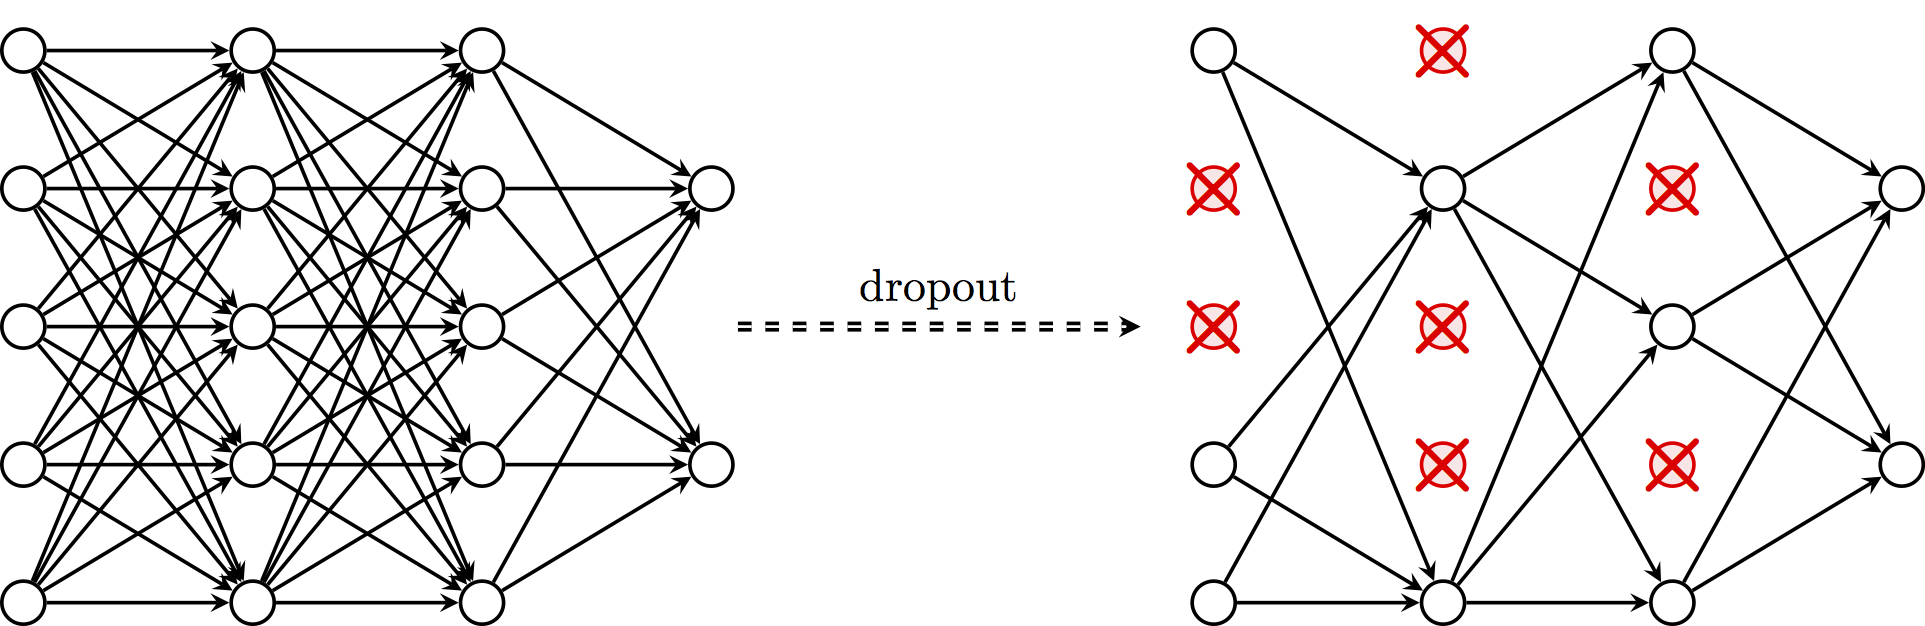
\includegraphics[width=\textwidth, height=0.3\textheight]{Figures/dropout}
	\caption{Left: neural network before dropout. Right: neural network after dropout.}
	\label{fig:dropout}
\end{figure}   

While a neural network learns, neuron weights settle into their context within the network. Those weights are tuned for specific features providing some specialization. However, neighboring neurons become to rely on this specialization, which, if taken too far, can result in a fragile model too specialized on the training data. Hence, if neurons are randomly dropped out of the network during training, other neurons will have to step in and handle the representation required to make predictions for the missing neurons. This is believed to result in multiple independent internal representations being learned by the network. The effect is that the network becomes less sensitive to the specific weights of neurons and results in a model capable of better generalization and less likely to overfit the training data.    

The output layer is composed of one sigmoid node that returns a value between 0 and 1 corresponding to the final score prediction. The class of the site is determined by the output of this neuron:

\[class(i) = 
\begin{cases} 
	1 & \text{if } o \geq 0.4 \\
	0 & \text{if } o < 0.4
\end{cases}
\]

Where $i$ and $o$ denote respectively the input and the output of the network. The prediction threshold value $0.4$ has been empirically evaluated. 


\begin{figure}[hbt!]
	\centering
	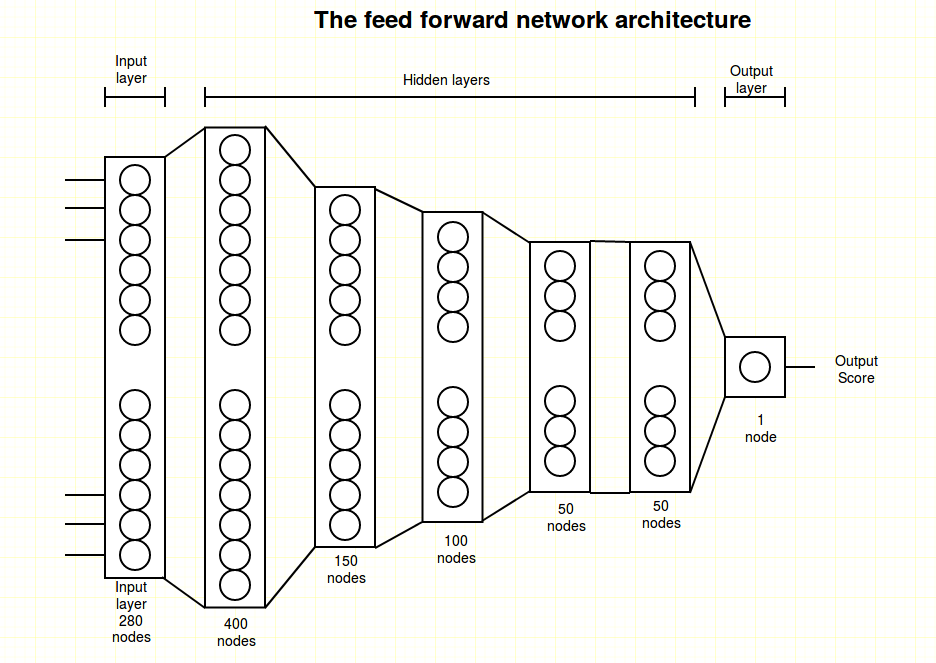
\includegraphics[width=\textwidth, height=0.52\textheight]{Figures/NN}
	\caption{\textbf{The feed-forward neural network}. The first hidden layer increases the dimensionality of the input allowing the representation of data in a more complex feature space. There is debate in the machine learning community regarding the need of such over-completion layers, as they do not necessarily improve the accuracy whilst making the learning process slower. Considering that the relatively low number of inputs of the proposed network allows a fast training procedure, we opted to include this higher dimension layer to give the network the chance of identifying more complex patterns.}
	\label{fig:NN}
\end{figure}

For the loss function we chose the binary cross entropy with Adam optimizer set with the following parameters:

\begin{itemize}
	\item learning rate = 0.002;
	\item beta\_1 = 0.9;
	\item beta\_2 = 0.999;
	\item epsilon = $1e-8$;
	\item decay = 0.0
\end{itemize}

The resulting architecture can be visualized in figure\ref{fig:NN} and parameters such as number of layers and neurons have been chosen through cross validation.

Despite being a very simple model, this network showed a better performances on the test set compared to other deeper (that is with more hidden layers) or more complex (i.e with a greater number of nodes) models. Check chapter \ref{Chapter5} for further details on the results.

\section{The Convolutional Neural Network aka CNN}
We have explained earlier, that the second encoding function provided by DeepMiRNA is based on Dna2Vec \cite{dna_distributed_repr}. In computational biology, one of the ubiquitous representation of long DNA sequence is dividing it into shorter k-mer components.  Unfortunately, the straightforward vectorization of k-mer as a one-hot vector is vulnerable to the curse of dimensionality. Worse yet, the distance between any pair of one-hot vectors is equidistant, even though, for example, the sequence \emph{ATGGC} should be closer to \emph{ATGGG} than \emph{CACGA}. This might be particularly problematic when applying the latest machine learning algorithms to solve problems in biological sequence analysis. Dna2Vec is, thus, a distributed representation of biological sequences that allows mapping k-mers to vectors of real numbers. By splitting the miRNA:MBS duplex in a fixed number of variable length k-mers, we were able to encode each pair into a bi-dimensional matrix. 

More specifically, each k-mer is embedded into a continuous vector space of $100$ dimensions, and each duplex is divided into 9 variable length k-mers: concatenating these vectors we obtain a $9x100$ matrix representing the encoded sequence (see figure \ref{fig:dna_embedding}).

\begin{figure}[hbt!]
	\centering
	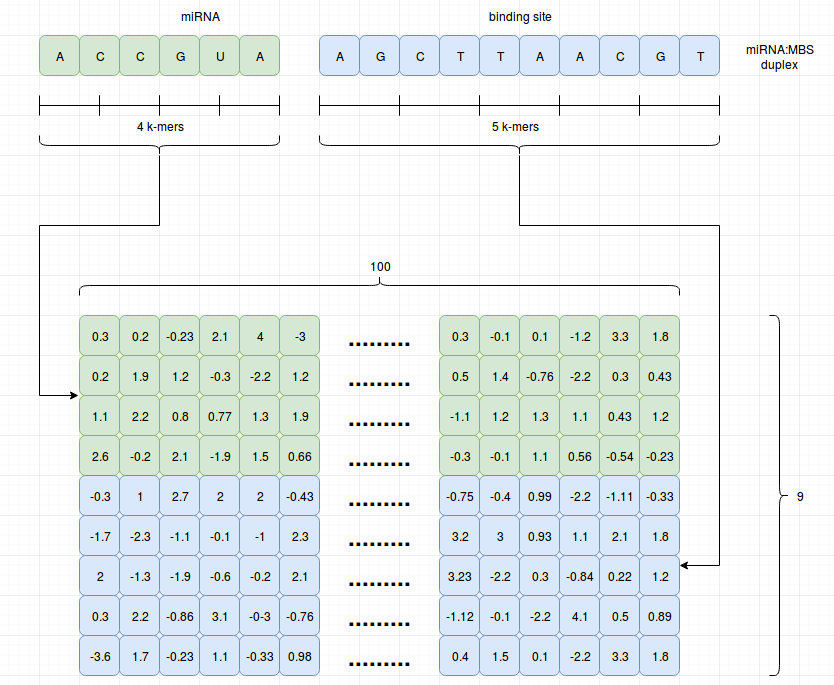
\includegraphics[width=\textwidth, height=0.4\textheight]{Figures/dna_embedding}
	\caption{\textbf{Sequence Embedding.} In green the miRNA sequence is split into 4 k-mers each mapped in a 100-dimension vector. In blue the same is done with miRNA binding site which is divided into 5 k-mers. The concatenation of the 9 resulting vectors is the matrix distributed representation of the duplex.}
	\label{fig:dna_embedding}
\end{figure}

With this representation, we believe the best base model to use for our task is represented by a convolutional neural network. 

\subsection{CNN architecture}


  


	% Chapter 5

\chapter{Neural network design and implementation} % Main chapter title

\label{Chapter5} % For referencing the chapter elsewhere, use \ref{Chapter5} 

%----------------------------------------------------------------------------------------
\section{External libraries}
DeepMiRNA has been developed using \emph{Python3}. The \emph{requirements.txt} file, present in the project root directory, contains names and versions of all libraries used for the implementation. In particular, we used \emph{Pandas} and \emph{Numpy} for the preprocessing step and the datasets preparation together with \emph{RNA} (the Python version of the Vienna Cofold) and \emph{Biopython} to parse .fasta files and convert them to .csv. 

Implementation of the neural network was done with \emph{Keras}\cite{keras} using \emph{Tensorflow} backend\cite{tensorflow}. Keras is an open-source neural-network library capable of running on top of TensorFlow, Theano and other major deep learning frameworks. Keras contains numerous implementations of commonly used NN building blocks such as layers, optimizers or activation functions and it aims at being user-friendly, modular and extensible. However, Keras, which is now fully supported in the Tensorflow's core library, has been conceived more as an interface than a standalone framework. 

We opted for the use of this library because it offers a higher-level, more intuitive set of abstractions that makes it easier to develop deep learning models.    

\section{Choosing the right model}
Building deep learning applications in the real world is a never-ending process of selecting and refining the right elements for a specific solution. Among those elements, the selection of the correct model and the right structure of the training dataset are, arguably, the two most important decisions that any data scientist needs to make when designing deep learning solutions. How to decide what deep learning model to use for a specific problem? How do we know whether we are using the correct training dataset or we should gather more data? Those questions are the common denominator across all stages of the life cycle of a deep learning application. Even though there is no magic answer to those questions, there are several ideas that could guide the decision process. 

First of all, we need to start identifying the correct baseline model, in particular, we should select what type of networks suits more the input dataset. In the case of miRNA target predictions, the topological structure of the available data is strictly correlated to the vectorization method selected. If we opt for the one-hot encoding that maps duplexes into fixed-size vectors, we should be thinking of using an MLP network with interlayer connectivity. While, if we select the Dna2Vec approach that transforms each duplex into a matrix, then the problem could be tackled using convolutional neural networks (CNN)\cite{dl}.  

The second part concerns the selection of the optimization algorithm to use. The most popular are, arguably, SGD (Stochastic Gradient Descent) and its variation using momentum or learning decay, and Adam. The latter, in particular, is very often used combined with CNN.

As mentioned in chapter \ref{Chapter4} DeepMiRNA uses 2 different neural networks for the training stage according to the chosen data representation: a regular feed-forward network for the one-hot encoded sequences and a CNN for the Dna2Vec encoded duplexes. 

\section{The feed-forward network} 
The MLP network we designed for the miRNA target prediction task is a very simple neural network consisting of 5 dense hidden layers, comprising rectifier activation function ReLU nodes, each followed by a dropout layer. Dropout \cite{dropout} is a regularization technique used to prevent overfitting. In this thesis, the dropout rate has been set to $0.7$ meaning that there is a probability $p = 0.3$ that a certain neuron is ignored (i.e set to 0). Basically, this implies that their contribution to the activation of downstream (i.e. next layer) neurons is temporally removed on the forward pass and weight update is not applied on the backward pass (see figure \ref{fig:dropout}).

\begin{figure}[hbt!]
	\centering
	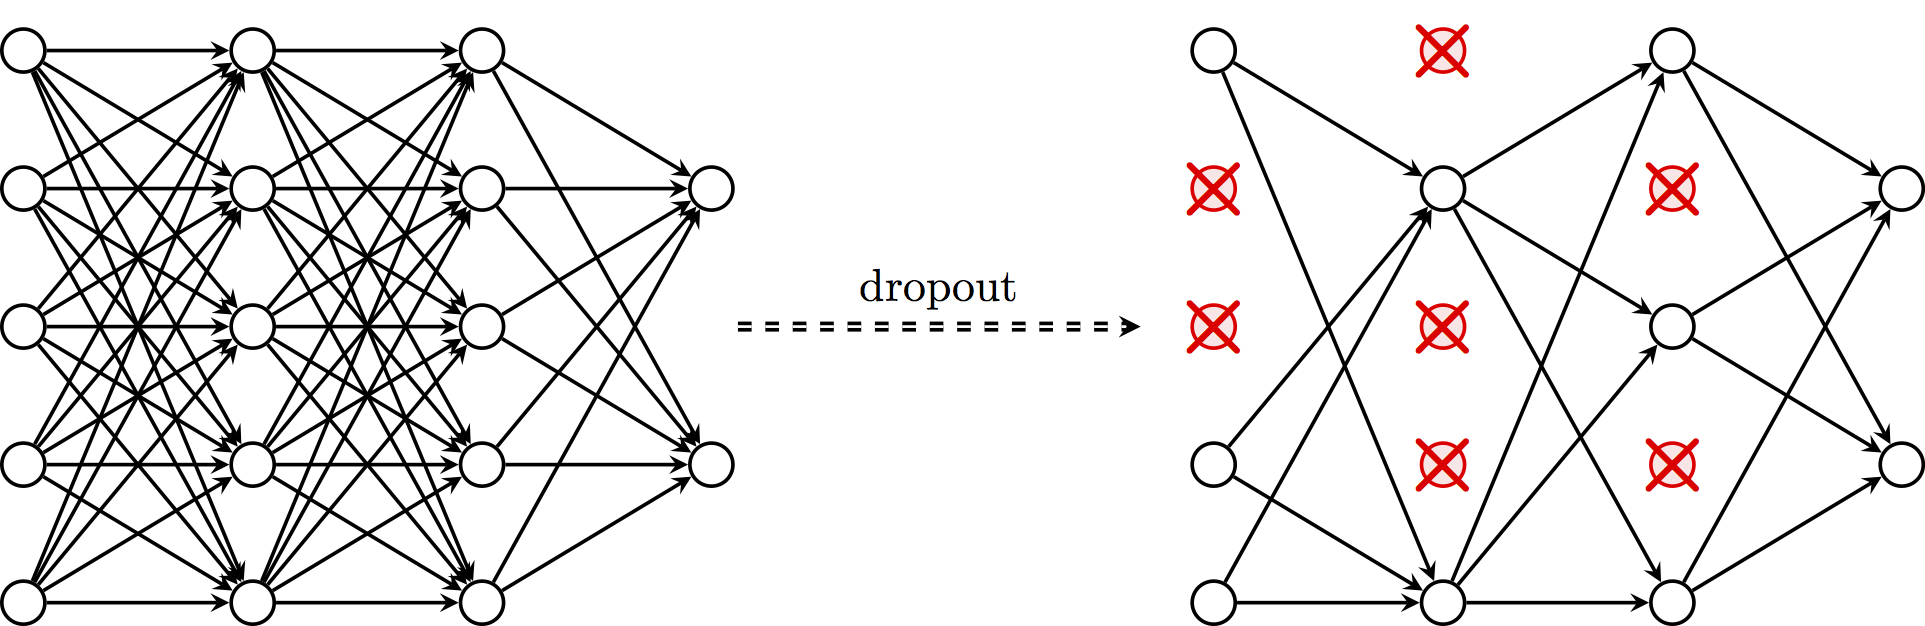
\includegraphics[width=\textwidth, height=0.3\textheight]{Figures/dropout}
	\caption{\keyword{Dropout.} Left: neural network before dropout. Right: neural network after dropout.}
	\label{fig:dropout}
\end{figure}   

While a neural network learns, neuron weights settle into their context within the network. Those weights are tuned for specific features providing some specialization. However, neighboring neurons become to rely on this specialization, which, if taken too far, can result in a fragile model with a reduced generalization capability. Hence, if neurons are randomly dropped out of the network during training, other neurons will have to step in and handle the representation required to make predictions for the missing neurons. This is believed to result in multiple independent internal representations being learned by the network. The effect is that the network becomes less sensitive to the specific weights of neurons and results in a model capable of better generalization and less likely to overfit the training data.    

The output layer is composed of one sigmoid node that returns a value between 0 and 1 corresponding to the final score prediction. The class of the site is determined by the output of this neuron:

\[class(i) = 
\begin{cases} 
	1 & \text{if } o \geq 0.4 \\
	0 & \text{if } o < 0.4
\end{cases}
\]

Where $i$ and $o$ denote respectively the input and the output of the network. The prediction threshold value $0.4$ has been empirically evaluated. 


\begin{figure}[hbt!]
	\centering
	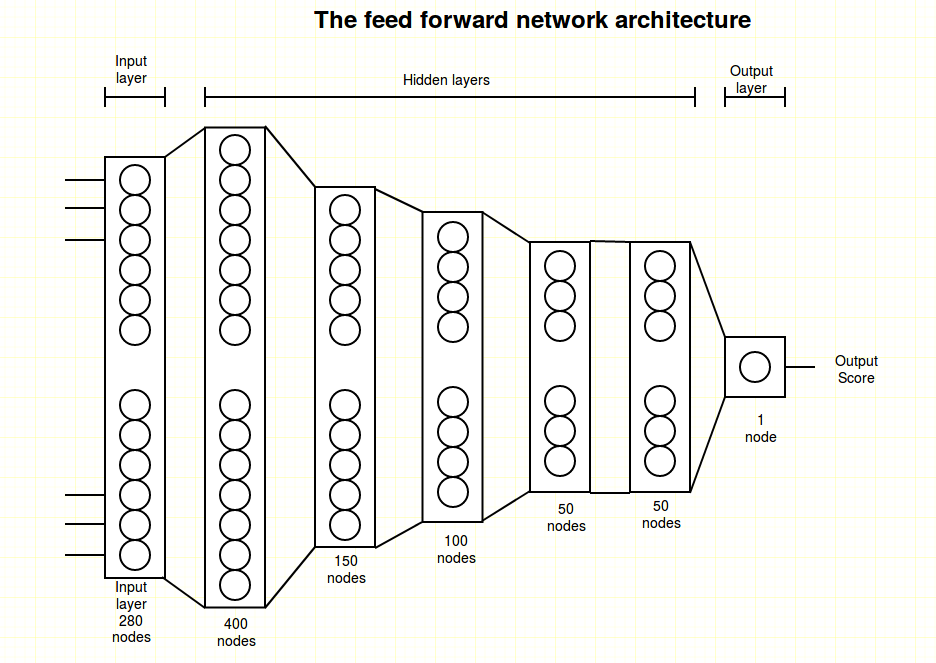
\includegraphics[width=\textwidth, height=0.52\textheight]{Figures/NN}
	\caption{\textbf{The feed-forward neural network}. The first hidden layer increases the dimensionality of the input allowing the representation of data in a more complex feature space. There is a debate in the machine learning community regarding the need for such over-completion layers, as they do not necessarily improve the accuracy whilst making the learning process slower. Considering that the relatively low number of inputs of the proposed network allows a fast training procedure, we opted to include this higher dimension layer to give the network the chance of identifying more complex patterns.}
	\label{fig:NN}
\end{figure}

As loss function, we chose the binary cross entropy with Adam optimizer set with the following parameters:

\begin{itemize}
	\item learning rate = 0.002;
	\item beta\_1 = 0.9;
	\item beta\_2 = 0.999;
	\item epsilon = $1e-8$;
	\item decay = 0.0
\end{itemize}

The resulting architecture can be visualized in figure\ref{fig:NN} and parameters, such as the number of layers and neurons, have been chosen through cross-validation.

Despite being a very simple model, this network showed better performances on the test set compared to other deeper (that is with more hidden layers) or more complex (i.e with a greater number of nodes) models. Check chapter \ref{Chapter6} for further details on the results.

\section{The Convolutional Neural Network aka CNN}
We have explained earlier, that the second encoding function provided by DeepMiRNA is based on Dna2Vec \cite{dna_distributed_repr}. In computational biology, one of the most widely used representations for long DNA sequences consists in dividing the transcript into shorter k-mer components.  Unfortunately, the straightforward vectorization of k-mer as a one-hot vector is vulnerable to the curse of dimensionality. Worse yet, the distance between any pair of one-hot vectors is equidistant, even though, for example, the sequence \emph{ATGGC} should be closer to \emph{ATGGG} than \emph{CACGA}. This might be particularly problematic when applying the latest machine learning algorithms to solve problems in biological sequence analysis. Dna2Vec is, thus, a distributed representation of biological sequences that allows mapping k-mers to dense vectors of real numbers. By splitting the miRNA:MBS duplex in a fixed number of variable length k-mers, we were able to encode each pair into a bi-dimensional matrix. 

More specifically, each k-mer is embedded into a continuous vector space of $100$ dimensions, and each duplex is divided into 9 variable length k-mers: concatenating these vectors we obtain a $9x100$ matrix representing the encoded sequence (see figure \ref{fig:dna_embedding}).

\begin{figure}[hbt!]
	\centering
	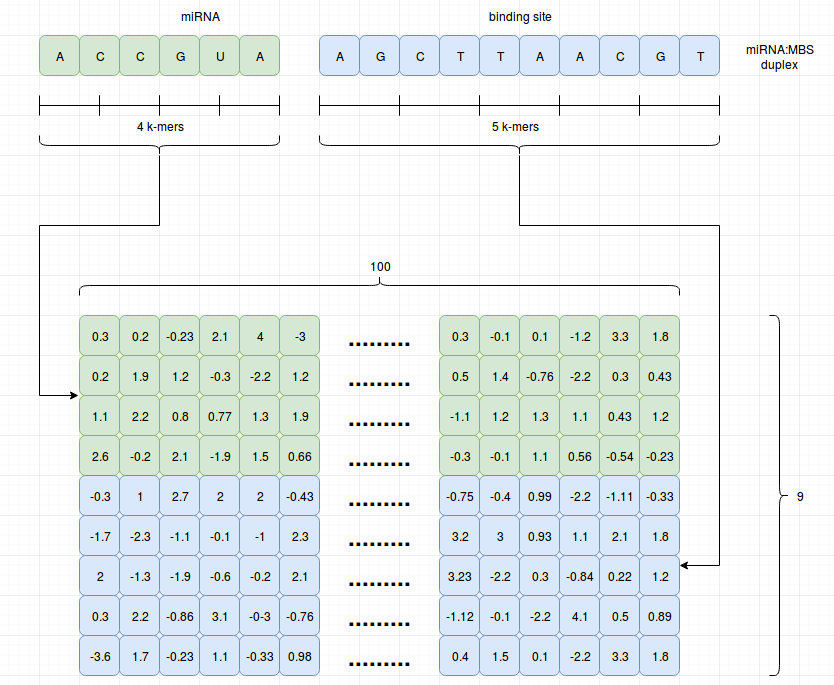
\includegraphics[width=\textwidth, height=0.4\textheight]{Figures/dna_embedding}
	\caption{\textbf{Sequence Embedding.} In green the miRNA sequence is split into 4 k-mers each mapped in a 100-dimension vector. In blue the same is done with miRNA binding site which is divided into 5 k-mers. The concatenation of the 9 resulting vectors is the matrix distributed representation of the duplex.}
	\label{fig:dna_embedding}
\end{figure}

With this representation, we believe the best base model to use for our task is represented by a convolutional neural network. 

\subsection{CNN architecture}
Once the baseline model has been chosen, one must proceed with its implementation selecting the best possible design. This step can be very tricky, especially when dealing with convolutional networks.  In fact, according to the complexity of the architecture and the representation of the available data, a CNN may require a long training time, with a great number of epochs. This makes the evaluation of the model design a complicated task: large validation errors and little improvements in the first few epochs does not always imply that the chosen architecture is wrong.   

For DeepMiRNA, the network was configured so that the number of inputs in the input layer was equal to the dimensionality of the encoded sequences,  while the output layer consisted of two softmax neurons. 

The architecture of our convolutional network is shown in figure \ref{fig:cnn} and it is mainly inspired to the CNN used in \cite{cnn_arch}. Given that our model must be trained on a relatively small dataset we decided to adopt a single level of convolutional feature map followed by a non-linear ReLU activation layer and a max pooling layer immediately preceding the output softmax neurons. 

\begin{figure}[hbt!]
	\centering
	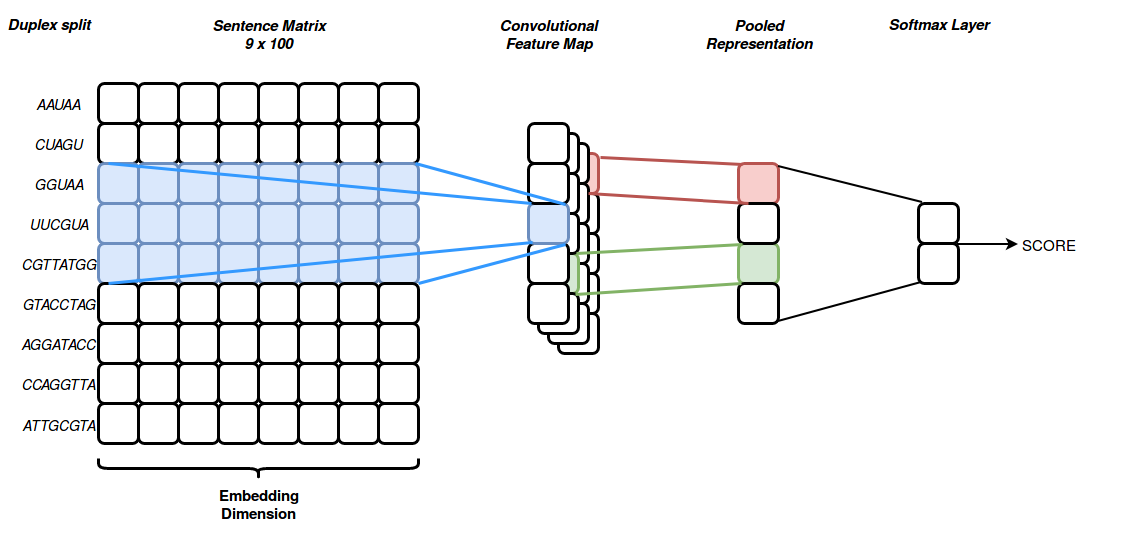
\includegraphics[width=\textwidth, height=0.4\textheight]{Figures/cnn_arch}
	\caption{\textbf{CNN architecture.} The input duplex is first split in 9 different length kmers to form the sentence matrix. The matrix is then fed into the convolutional network for prediction.}
	\label{fig:cnn}
\end{figure}     

For the compiling step required for the training stage, we selected the binary cross entropy loss function and we set the Adam optimizer with the same parameters used for the MLP network.

Despite showing discrete results in terms of accuracy and F1-score on the validation set composed of never seen miRNA:MBS examples, the CNN does not perform very well on the test set especially if compared to the feed-forward network. The main issue
concerns its scarce ability in correctly identifying negative miRNA:mRNA pairs. This fact, unfortunately, prevents this model from having a good generalization. We believe the main reason behind this, it's most likely due to the very small amount of negatively validated entries in the training set: issue that, instead, does not seem to affect the MLP model performance.

  


%---------------------------------------------------------------------------------------
%
%	THESIS CONTENT - APPENDICES
%
%---------------------------------------------------------------------------------------
	
	\appendix % Cue to tell LaTeX that the following "chapters" are Appendices
	% Appendix A

\chapter{Frequently Asked Questions} % Main appendix title

\label{AppendixA} % For referencing this appendix elsewhere, use \ref{AppendixA}

\section{How do I change the colors of links?}

The color of links can be changed to your liking using:

{\small\verb!\hypersetup{urlcolor=red}!}, or

{\small\verb!\hypersetup{citecolor=green}!}, or

{\small\verb!\hypersetup{allcolor=blue}!}.

\noindent If you want to completely hide the links, you can use:

{\small\verb!\hypersetup{allcolors=.}!}, or even better: 

{\small\verb!\hypersetup{hidelinks}!}.

\noindent If you want to have obvious links in the PDF but not the printed text, use:

{\small\verb!\hypersetup{colorlinks=false}!}.


%---------------------------------------------------------------------------------------%
%	BIBLIOGRAPHY
%
%---------------------------------------------------------------------------------------

	\bibliography{biblio}
	\bibliographystyle{acm}

%----------------------------------------------------------------------------------------

\end{document}  
